\documentclass[a4paper,12pt,halfparskip,DIV14]{scrartcl}

\newcommand{\dokumenttitel}{Design}
\usepackage{../bodesuri}
\usepackage{multicol}


\begin{document}

\title{\dokumenttitel}
\titlehead{
	\centering
	
\includegraphics[width=0.5 \textwidth, clip, trim = 0 7cm 0 0]{design/externes_design/bodesuri_plakat}
	\vspace{2cm}
}
\author{Danilo~Couto, Philippe~Eberli, \\ Pascal~Hobus, Reto~Schüttel, Robin~Stocker}
\maketitle
\newpage

\pagenumbering{roman}

\tableofcontents
\thispagestyle{plain}
\newpage

\pagenumbering{arabic}

\markright{Bodesuri -- \dokumenttitel}


\section{Architektur} % (fold)
\label{sec:architektur}
\subsection{Architektonische Darstellung } % (fold)
\label{sub:architektonische_darstellung_}
Beschreibt die Softwarearchitektur eines Systems und wie sie sich präsentiert.
% subsection architektonische_darstellung_ (end)

\subsection{Architektonische Ziele \& Einschränkungen} % (fold)
\label{sub:architektonische_ziele_einschränkungen}
Beschreibt die Softwareanforderungen und Objekte, welche einen Einfluss auf die Architektur haben [Bspl: Safety, Security, Privacy, Distribution, …] Beinhaltet auch eine Beschreibung von Design und Implementationsstrategie, Teamstruktur, Entwicklungstools, Zeitplan, etc…
% subsection architektonische_ziele_einschränkungen (end)

\newpage
\subsection{Logische Architektur} % (fold)
\label{sub:logische_architektur}

\subsubsection{Legende für die verwendeten Farben in den Diagrammen}\label{ssub:legende} % (fold)
\begin{figure}
	[htp] \centering 
	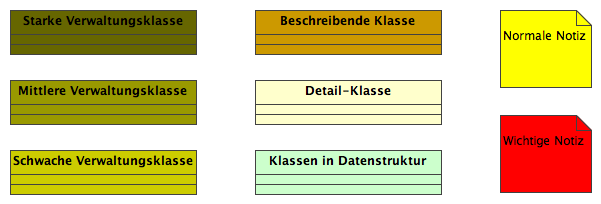
\includegraphics[width=1\textwidth]{legende.png} \caption{Legende für Diagrammfarben}\label{fig:legende.png} 
\end{figure}
% subsubsection legende (end)

\newpage
Beschreibung der logischen Struktur des Projekts
\begin{figure}
	[htp] \centering 
	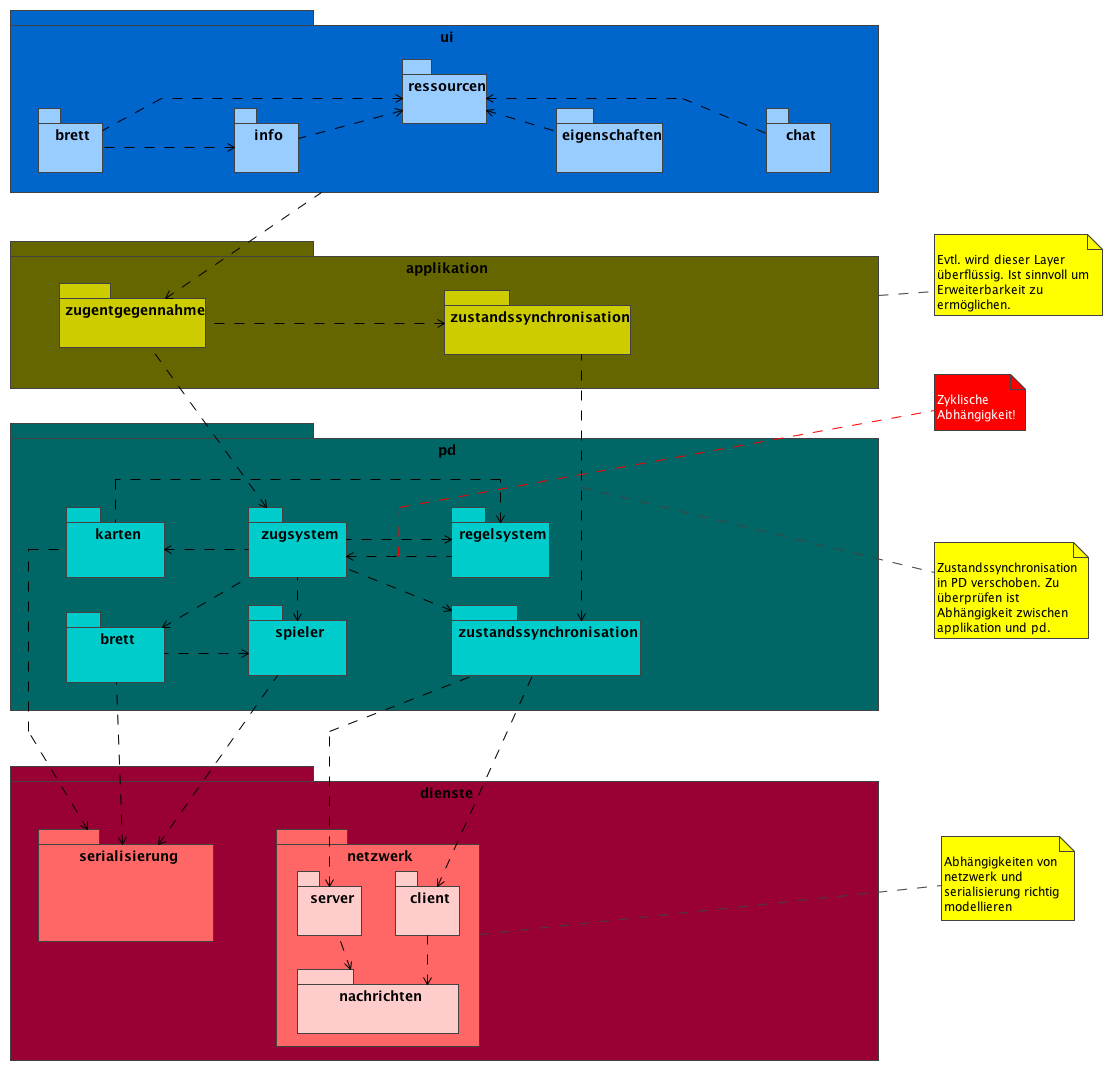
\includegraphics[width=1\textwidth]{Architektur.png} \caption{Architektur}\label{fig:Architektur.png} 
\end{figure}
\subsubsection{Übersicht} % (fold)
\label{ssub:Übersicht}
Beschreibung mit Text und Diagramm der Architektur. Aufteilung in Packages (zum Beispiel: 3-Layer-Architektur mit  GUI, Problem Domain und Datenhaltung)
% subsubsection Übersicht (end)

\subsubsection{Design Pakete} % (fold)
\label{ssub:design_pakete}
Für jedes definierte Package erfolgt eine Beschreibung mit Diagramm.

\paragraph{Package pd:} % (fold)
\label{ssub:package_pd}
\subparagraph{Beschreibung des Packages} % (fold)
\label{ssub:beschreibung_des_packages}
Beschreibung des Package. Aufgabe, etc…
% subparagraph beschreibung_des_packages (end)
\subparagraph{Diagramme} % (fold)
\label{ssub:diagramme}
Klassendiagramm
% subparagraph diagramme (end)
\subparagraph{Schnittstellen} % (fold)
\label{ssub:schnittstellen}
Beschreibung der Schnittstellen
% subparagraph schnittstellen (end)
\subparagraph{Operationen} % (fold)
\label{ssub:operationen}
Beschreibung der internen Operationen (evtl auch mit Sequendiagramm).
% subparagraph operationen (end)
% paragraph package_pd (end)

\newpage
\paragraph{Package pd.karten:} % (fold)
\label{ssub:package_pd_karten}
\subparagraph{Beschreibung des Packages} % (fold)
\label{ssub:beschreibung_des_packages}
Beschreibung des Package. Aufgabe, etc…
% subparagraph beschreibung_des_packages (end)
\subparagraph{Diagramme} % (fold)
\label{ssub:diagramme}
\begin{figure}
	[htp] \centering 
	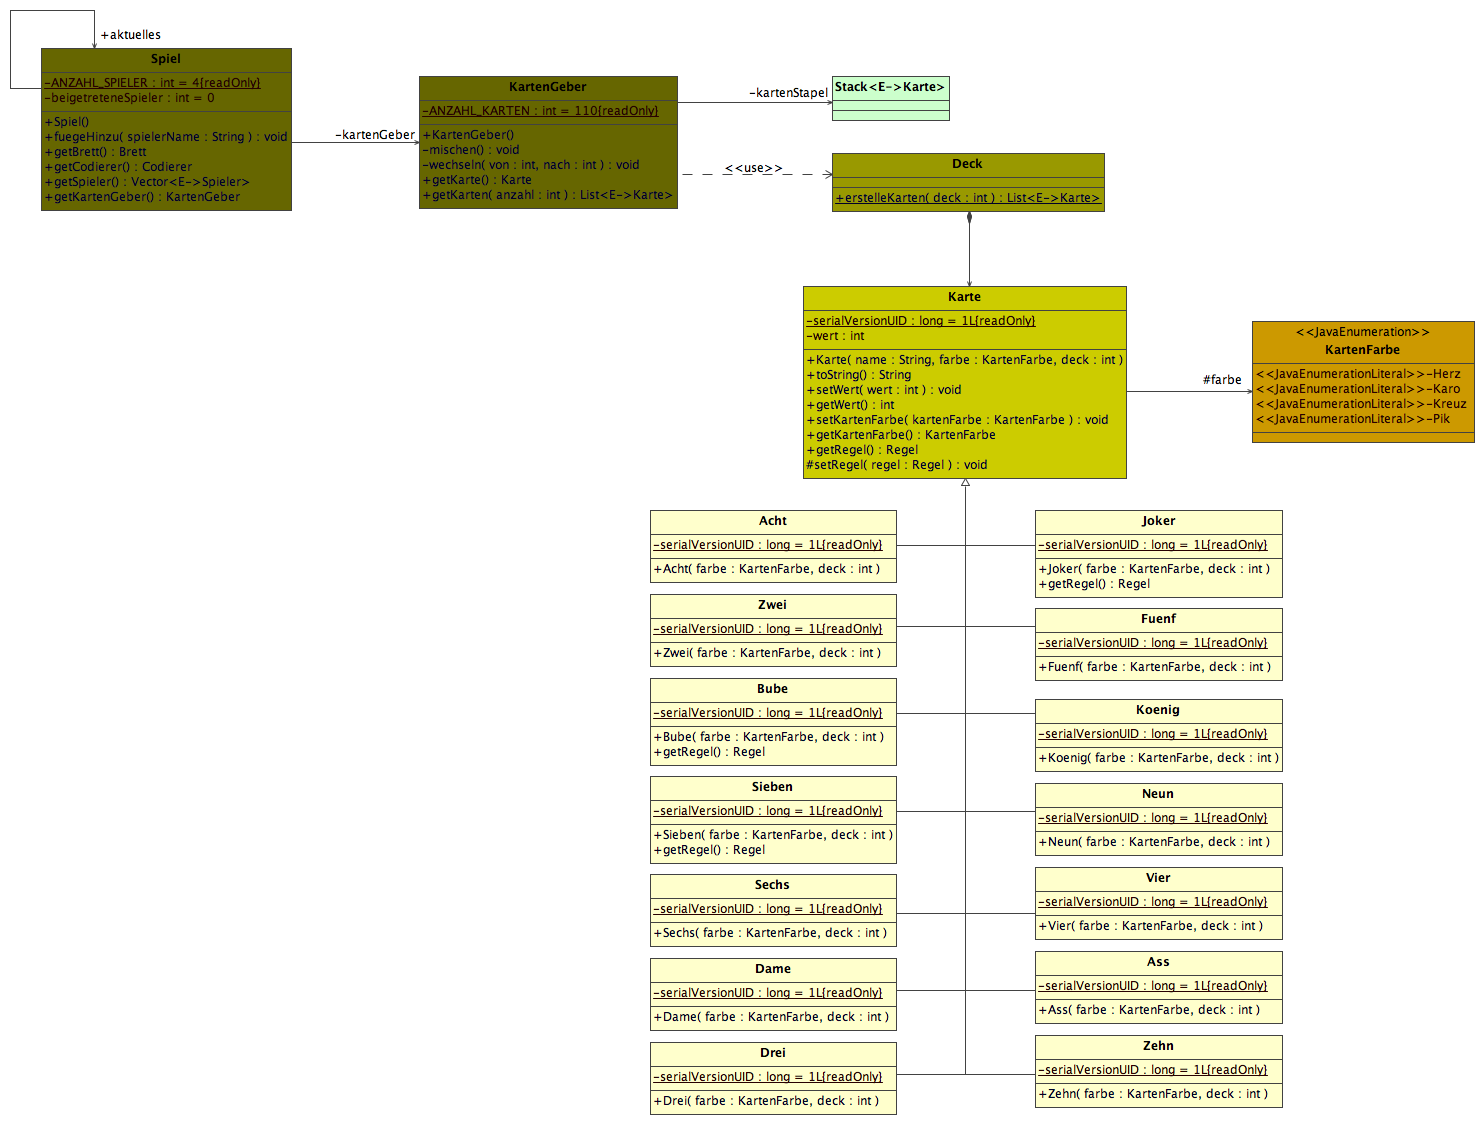
\includegraphics[width=1\textwidth]{pd_kartengeber.png} \caption{Kartengeber}\label{fig:pd_kartengeber.png} 
\end{figure}
% subparagraph diagramme (end)
\subparagraph{Schnittstellen} % (fold)
\label{ssub:schnittstellen}
Beschreibung der Schnittstellen
% subparagraph schnittstellen (end)
\subparagraph{Operationen} % (fold)
\label{ssub:operationen}
Beschreibung der internen Operationen (evtl auch mit Sequendiagramm).
% subparagraph operationen (end)
% paragraph package_pd_karten (end)

\newpage
\paragraph{Package pd.regelsystem, pd.zugsystem:} % (fold)
\label{ssub:package_pd_regelsystem}
\subparagraph{Beschreibung des Packages} % (fold)
\label{ssub:beschreibung_des_packages}
Beschreibung des Package. Aufgabe, etc…
% subparagraph beschreibung_des_packages (end)
\subparagraph{Diagramme} % (fold)
\label{ssub:diagramme}
\begin{figure}
	[htp] \centering 
	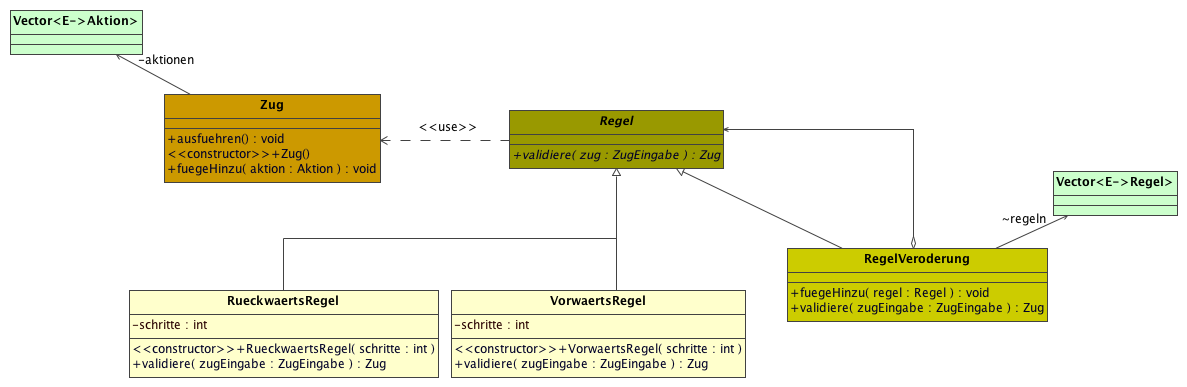
\includegraphics[width=1\textwidth]{pd_regelsystem.png} \caption{Regelsystem}\label{fig:pd_regelsystem.png} 
\end{figure}
% subparagraph diagramme (end)
\subparagraph{Schnittstellen} % (fold)
\label{ssub:schnittstellen}
Beschreibung der Schnittstellen
% subparagraph schnittstellen (end)
\subparagraph{Operationen} % (fold)
\label{ssub:operationen}
Beschreibung der internen Operationen (evtl auch mit Sequendiagramm).
\begin{figure}
	[htp] \centering 
	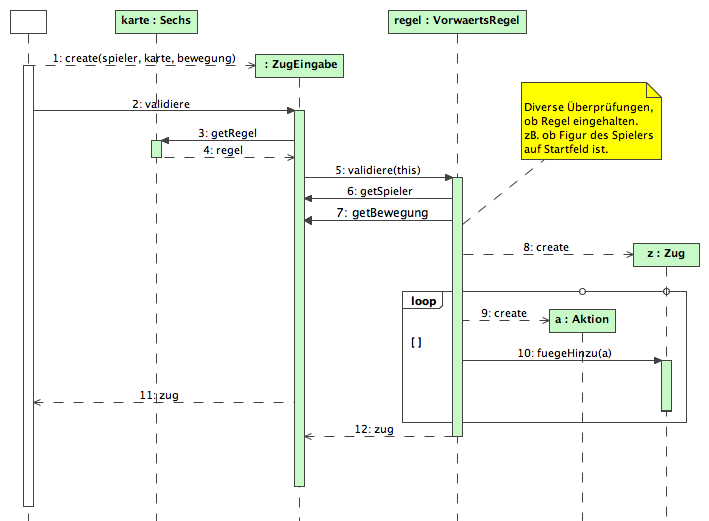
\includegraphics[width=1\textwidth]{pd_validierung.png} \caption{Validierung von Spielzügen}\label{fig:pd_validierung.png} 
\end{figure}
% subparagraph operationen (end)
% paragraph package_pd_regelsystem (end)

\newpage
\paragraph{Package pd.brett, pd.spieler:} % (fold)
\label{ssub:package_pd_brett}
\subparagraph{Beschreibung des Packages} % (fold)
\label{ssub:beschreibung_des_packages}
Beschreibung des Package. Aufgabe, etc…
% subparagraph beschreibung_des_packages (end)
\subparagraph{Diagramme} % (fold)
\label{ssub:diagramme}
\begin{figure}
	[htp] \centering 
	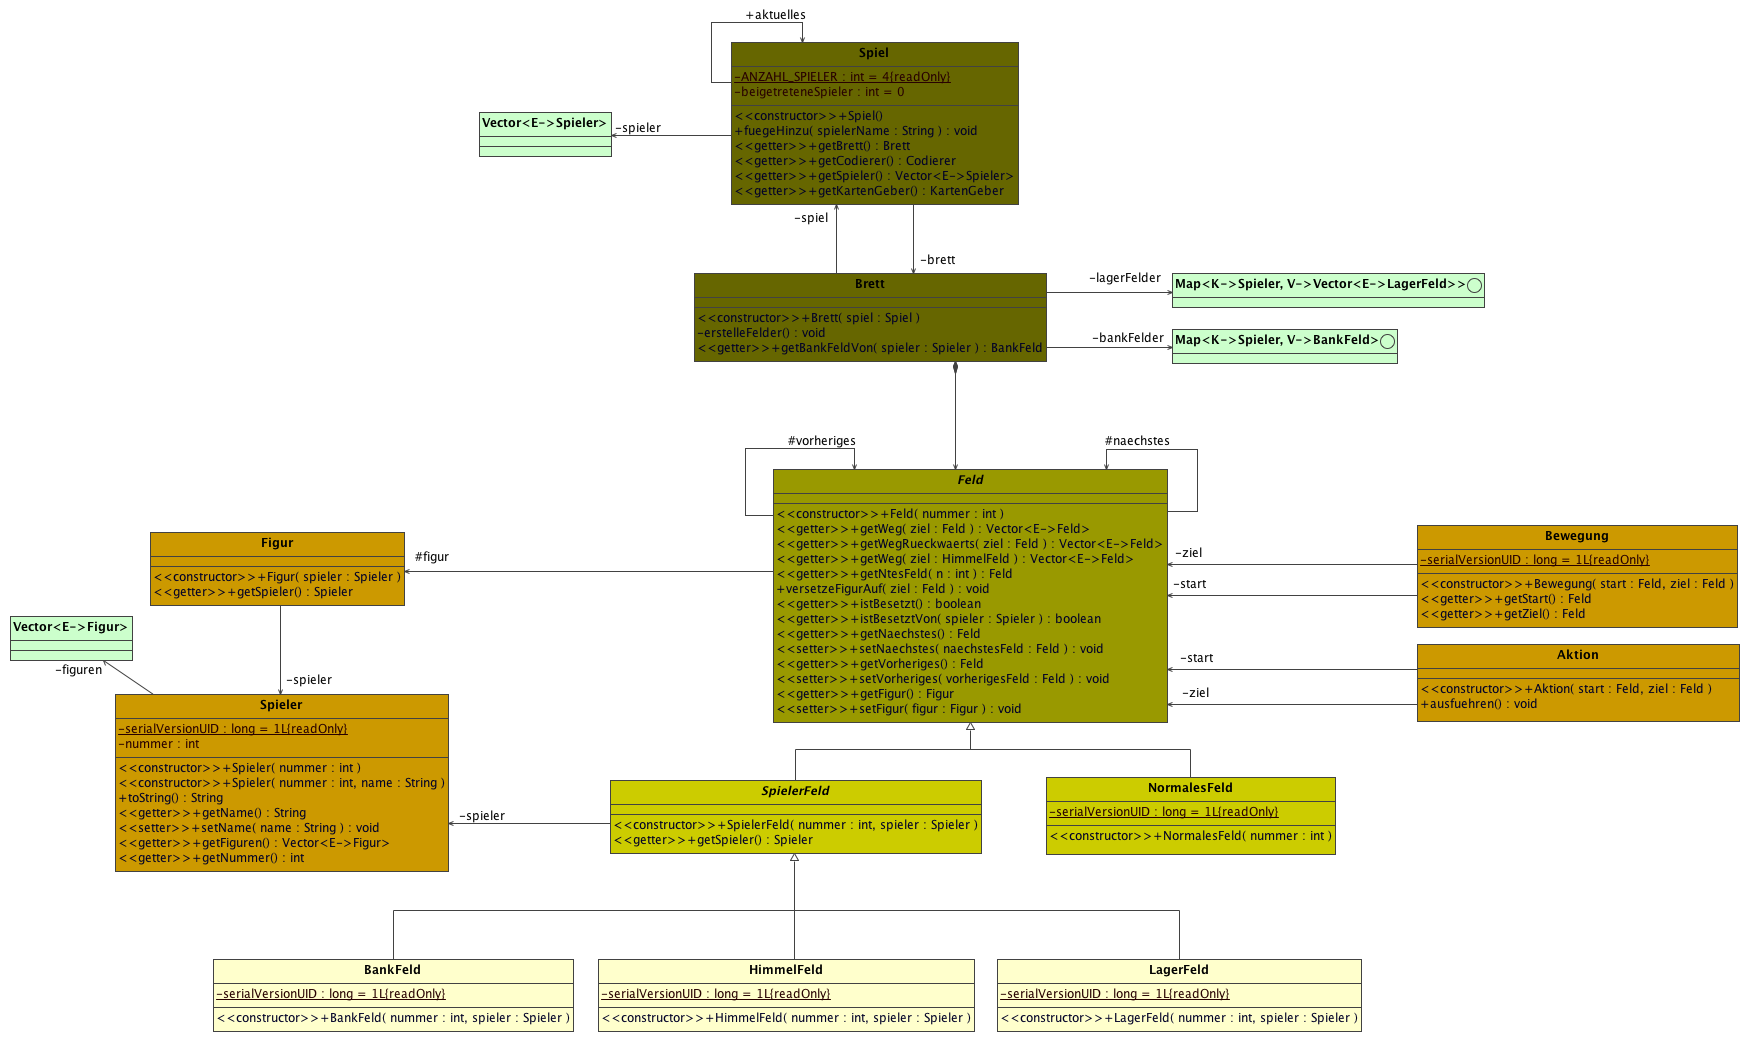
\includegraphics[width=1\textwidth]{pd_brett.png} \caption{Brett und Figuren}\label{fig:pd_brett.png} 
\end{figure}
% subparagraph diagramme (end)
\subparagraph{Schnittstellen} % (fold)
\label{ssub:schnittstellen}
Beschreibung der Schnittstellen
% subparagraph schnittstellen (end)
\subparagraph{Operationen} % (fold)
\label{ssub:operationen}
Beschreibung der internen Operationen (evtl auch mit Sequendiagramm).
% subparagraph operationen (end)
% paragraph package_pd_brett (end)

\newpage
\paragraph{Package pd.zustandsynchronisation:} % (fold)
\label{ssub:package_pd_zustandsynchronisation}
\subparagraph{Beschreibung des Packages} % (fold)
\label{ssub:beschreibung_des_packages}
Beschreibung des Package. Aufgabe, etc…
% subparagraph beschreibung_des_packages (end)
\subparagraph{Diagramme} % (fold)
\label{ssub:diagramme}
Klassendiagramm
% subparagraph diagramme (end)
\subparagraph{Schnittstellen} % (fold)
\label{ssub:schnittstellen}
Beschreibung der Schnittstellen
% subparagraph schnittstellen (end)
\subparagraph{Operationen} % (fold)
\label{ssub:operationen}
Beschreibung der internen Operationen (evtl auch mit Sequendiagramm).
% subparagraph operationen (end)
% paragraph package_pd_zustandsynchronisation (end)

\newpage
\paragraph{Package dienste:} % (fold)
\label{ssub:package_dienste}
\subparagraph{Beschreibung des Packages} % (fold)
\label{ssub:beschreibung_des_packages}
Beschreibung des Package. Aufgabe, etc…
% subparagraph beschreibung_des_packages (end)
\subparagraph{Diagramme} % (fold)
\label{ssub:diagramme}
Klassendiagramm
% subparagraph diagramme (end)
\subparagraph{Schnittstellen} % (fold)
\label{ssub:schnittstellen}
Beschreibung der Schnittstellen
% subparagraph schnittstellen (end)
\subparagraph{Operationen} % (fold)
\label{ssub:operationen}
Beschreibung der internen Operationen (evtl auch mit Sequendiagramm).
% subparagraph operationen (end)
% paragraph package_dienste (end)

\newpage
\paragraph{Package dienste.serialisierung:} % (fold)
\label{ssub:package_dienste_serialisierung}
\subparagraph{Beschreibung des Packages} % (fold)
\label{ssub:beschreibung_des_packages}
Beschreibung des Package. Aufgabe, etc…
% subparagraph beschreibung_des_packages (end)
\subparagraph{Diagramme} % (fold)
\label{ssub:diagramme}
Klassendiagramm
% subparagraph diagramme (end)
\subparagraph{Schnittstellen} % (fold)
\label{ssub:schnittstellen}
Beschreibung der Schnittstellen
% subparagraph schnittstellen (end)
\subparagraph{Operationen} % (fold)
\label{ssub:operationen}
Beschreibung der internen Operationen (evtl auch mit Sequendiagramm).
\begin{figure}
	[htp] \centering 
	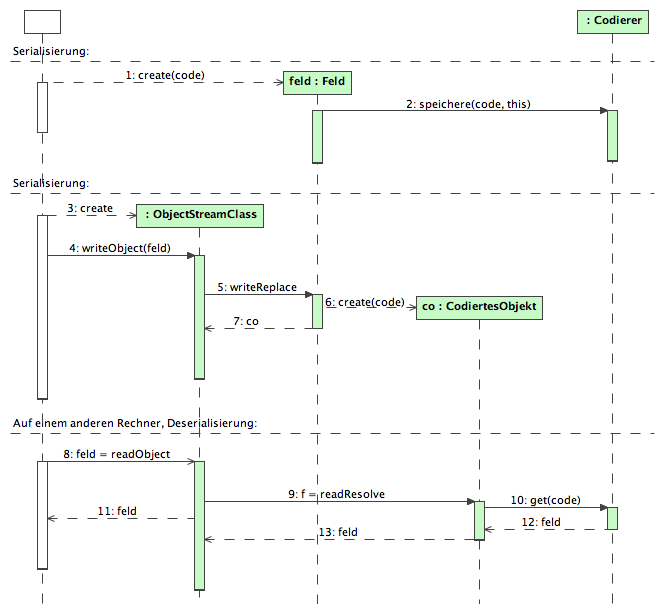
\includegraphics[width=1\textwidth]{dienste_serialisierung.png} \caption{Serialisierung}\label{fig:dienste_serialisierung.png} 
\end{figure}
% subparagraph operationen (end)
% paragraph package_dienste_serialisierung (end)

\newpage
\paragraph{Package dienste.netzwerk:} % (fold)
\label{ssub:package_dienste_netzwerk}
\subparagraph{Beschreibung des Packages} % (fold)
\label{ssub:beschreibung_des_packages}
Beschreibung des Package. Aufgabe, etc…
% subparagraph beschreibung_des_packages (end)
\subparagraph{Diagramme} % (fold)
\label{ssub:diagramme}
Klassendiagramm
% subparagraph diagramme (end)
\subparagraph{Schnittstellen} % (fold)
\label{ssub:schnittstellen}
Beschreibung der Schnittstellen
% subparagraph schnittstellen (end)
\subparagraph{Operationen} % (fold)
\label{ssub:operationen}
Beschreibung der internen Operationen (evtl auch mit Sequendiagramm).
\begin{figure}
	[htp] \centering 
	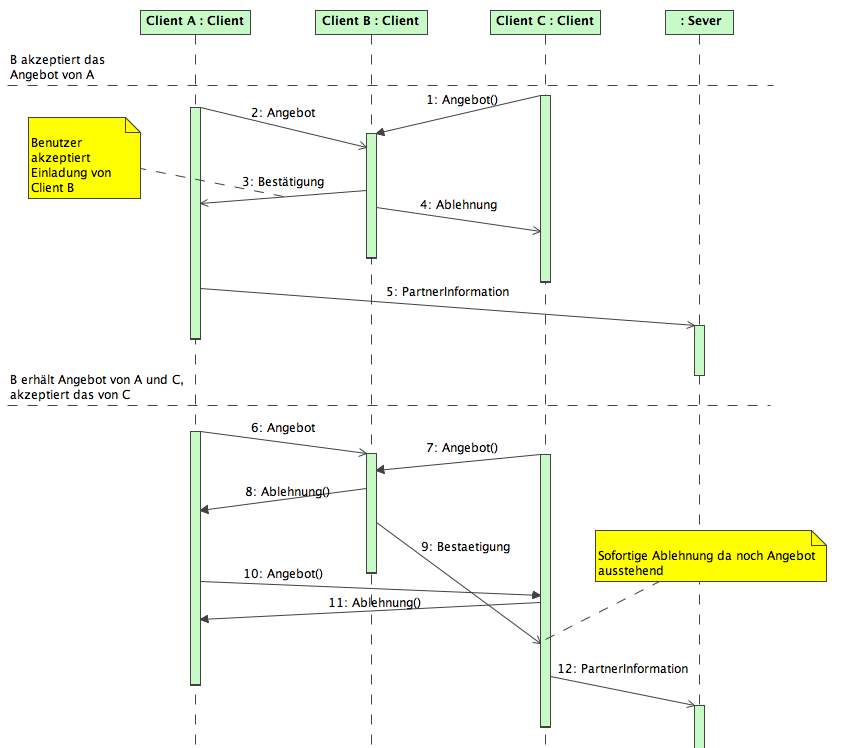
\includegraphics[width=1\textwidth]{dienste_partnerschaft_normal_1.png} \caption{Normale Partnerschaft - Teil 1 von 2}\label{fig:dienste_partnerschaft_normal_1.png} 
\end{figure}
\begin{figure}
	[htp] \centering 
	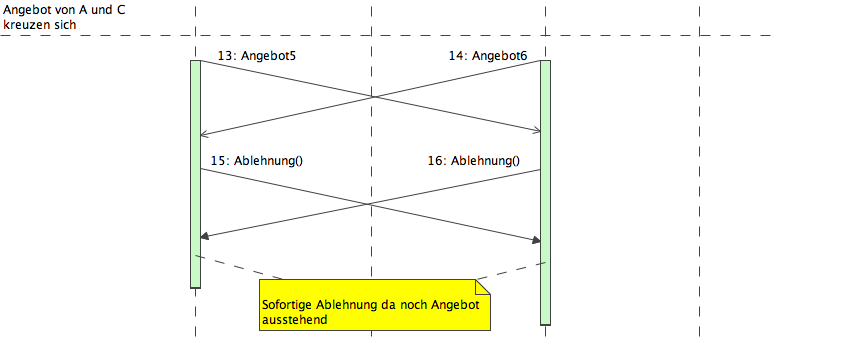
\includegraphics[width=1\textwidth]{dienste_partnerschaft_normal_2.png} \caption{Normale Partnerschaft - Teil 2 von 2}\label{fig:dienste_partnerschaft_normal_2.png} 
\end{figure}
\begin{figure}
	[htp] \centering 
	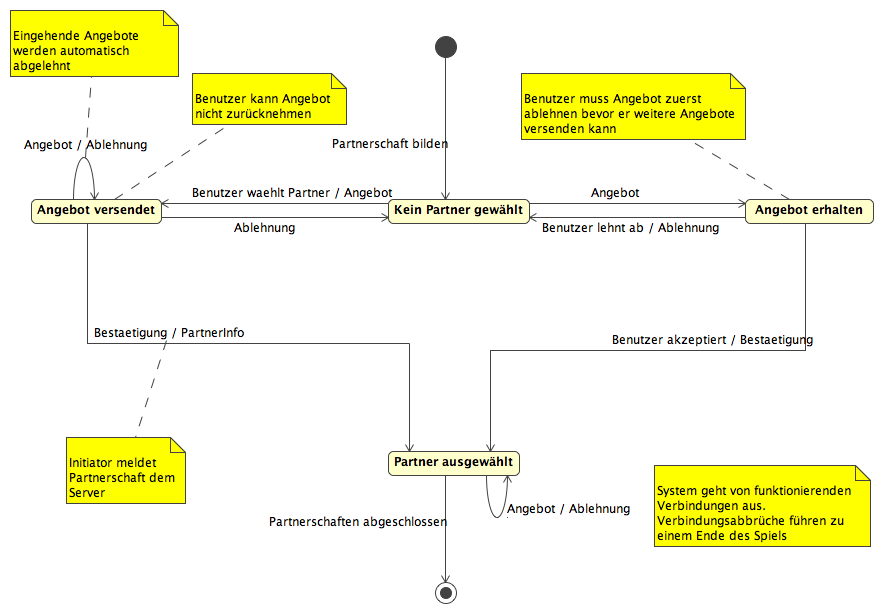
\includegraphics[width=1\textwidth]{dienste_partner.png} \caption{Partner Verhalten}\label{fig:dienste_partner.png} 
\end{figure}
\begin{figure}
	[htp] \centering 
	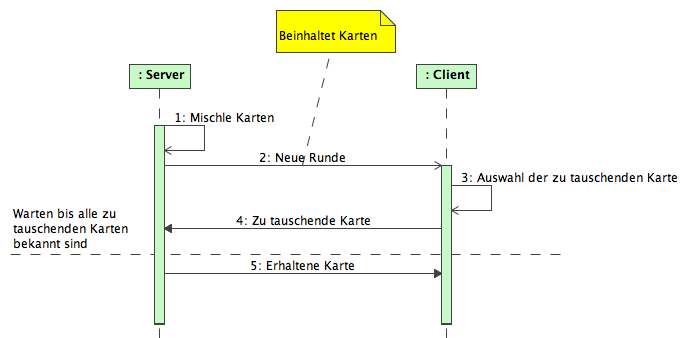
\includegraphics[width=1\textwidth]{dienste_rundenstart.png} \caption{Rundenstart}\label{fig:dienste_rundenstart.png} 
\end{figure}
\begin{figure}
	[htp] \centering 
	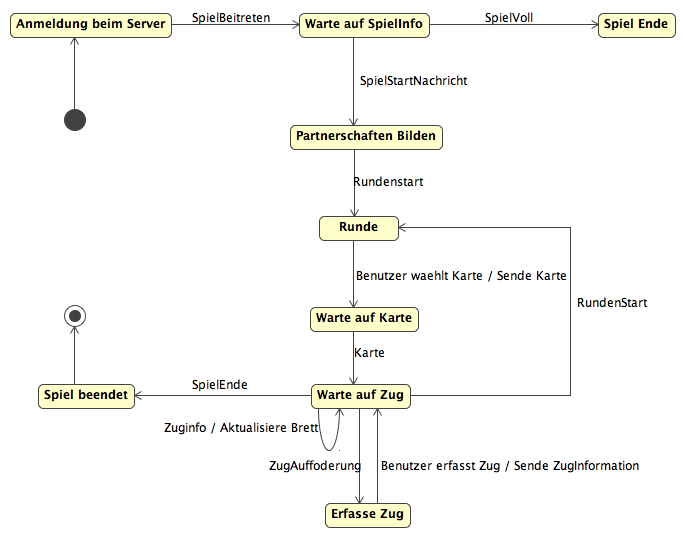
\includegraphics[width=1\textwidth]{dienste_client.png} \caption{Zustände des Client}\label{fig:dienste_client.png} 
\end{figure}
\begin{figure}
	[htp] \centering 
	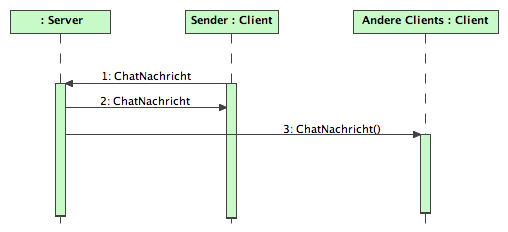
\includegraphics[width=1\textwidth]{dienste_chat.png} \caption{Chat Subsystem}\label{fig:dienste_chat.png} 
\end{figure}
% subparagraph operationen (end)
% paragraph package_dienste_netzwerk (end)

\newpage
\paragraph{Package ui:} % (fold)
\label{ssub:package_ui}
\subparagraph{Beschreibung des Packages} % (fold)
\label{ssub:beschreibung_des_packages}
Beschreibung des Package. Aufgabe, etc…
% subparagraph beschreibung_des_packages (end)
\subparagraph{Diagramme} % (fold)
\label{ssub:diagramme}
Klassendiagramm
% subparagraph diagramme (end)
\subparagraph{Schnittstellen} % (fold)
\label{ssub:schnittstellen}
Beschreibung der Schnittstellen
% subparagraph schnittstellen (end)
\subparagraph{Operationen} % (fold)
\label{ssub:operationen}
Beschreibung der internen Operationen (evtl auch mit Sequendiagramm).
% subparagraph operationen (end)
% paragraph package_ui (end)

\newpage
\paragraph{Package ui.brett:} % (fold)
\label{ssub:package_ui_brett}
\subparagraph{Beschreibung des Packages} % (fold)
\label{ssub:beschreibung_des_packages}
Beschreibung des Package. Aufgabe, etc…
% subparagraph beschreibung_des_packages (end)
\subparagraph{Diagramme} % (fold)
\label{ssub:diagramme}
Klassendiagramm
% subparagraph diagramme (end)
\subparagraph{Schnittstellen} % (fold)
\label{ssub:schnittstellen}
Beschreibung der Schnittstellen
% subparagraph schnittstellen (end)
\subparagraph{Operationen} % (fold)
\label{ssub:operationen}
Beschreibung der internen Operationen (evtl auch mit Sequendiagramm).
% subparagraph operationen (end)
% paragraph package_ui_brett (end)

\paragraph{Package ui.eigenschaften:} % (fold)
\label{ssub:package_ui_eigenschaften}
\subparagraph{Beschreibung des Packages} % (fold)
\label{ssub:beschreibung_des_packages}
Beschreibung des Package. Aufgabe, etc…
% subparagraph beschreibung_des_packages (end)
\subparagraph{Diagramme} % (fold)
\label{ssub:diagramme}
Klassendiagramm
% subparagraph diagramme (end)
\subparagraph{Schnittstellen} % (fold)
\label{ssub:schnittstellen}
Beschreibung der Schnittstellen
% subparagraph schnittstellen (end)
\subparagraph{Operationen} % (fold)
\label{ssub:operationen}
Beschreibung der internen Operationen (evtl auch mit Sequendiagramm).
% subparagraph operationen (end)
% paragraph package_ui_eigenschaften (end)

\newpage
\paragraph{Package ui.info:} % (fold)
\label{ssub:package_ui_info}
\subparagraph{Beschreibung des Packages} % (fold)
\label{ssub:beschreibung_des_packages}
Beschreibung des Package. Aufgabe, etc…
% subparagraph beschreibung_des_packages (end)
\subparagraph{Diagramme} % (fold)
\label{ssub:diagramme}
Klassendiagramm
% subparagraph diagramme (end)
\subparagraph{Schnittstellen} % (fold)
\label{ssub:schnittstellen}
Beschreibung der Schnittstellen
% subparagraph schnittstellen (end)
\subparagraph{Operationen} % (fold)
\label{ssub:operationen}
Beschreibung der internen Operationen (evtl auch mit Sequendiagramm).
% subparagraph operationen (end)
% paragraph package_ui_info (end)

\newpage
\paragraph{Package ui.ressourcen:} % (fold)
\label{ssub:package_ui_ressourcen}
\subparagraph{Beschreibung des Packages} % (fold)
\label{ssub:beschreibung_des_packages}
Beschreibung des Package. Aufgabe, etc…
% subparagraph beschreibung_des_packages (end)
\subparagraph{Diagramme} % (fold)
\label{ssub:diagramme}
Klassendiagramm
% subparagraph diagramme (end)
\subparagraph{Schnittstellen} % (fold)
\label{ssub:schnittstellen}
Beschreibung der Schnittstellen
% subparagraph schnittstellen (end)
\subparagraph{Operationen} % (fold)
\label{ssub:operationen}
Beschreibung der internen Operationen (evtl auch mit Sequendiagramm).
% subparagraph operationen (end)
% paragraph package_ui_ressourcen (end)

\newpage
\paragraph{Package applikation:} % (fold)
\label{ssub:package_applikation}
\subparagraph{Beschreibung des Packages} % (fold)
\label{ssub:beschreibung_des_packages}
Beschreibung des Package. Aufgabe, etc…
% subparagraph beschreibung_des_packages (end)
\subparagraph{Diagramme} % (fold)
\label{ssub:diagramme}
Klassendiagramm
% subparagraph diagramme (end)
\subparagraph{Schnittstellen} % (fold)
\label{ssub:schnittstellen}
Beschreibung der Schnittstellen
% subparagraph schnittstellen (end)
\subparagraph{Operationen} % (fold)
\label{ssub:operationen}
Beschreibung der internen Operationen (evtl auch mit Sequendiagramm).
% subparagraph operationen (end)
% paragraph package_applikation (end)

\newpage
\paragraph{Package applikation.zugentgegennahme:} % (fold)
\label{ssub:package_applikation_zugentgegennahme}
\subparagraph{Beschreibung des Packages} % (fold)
\label{ssub:beschreibung_des_packages}
Beschreibung des Package. Aufgabe, etc…
% subparagraph beschreibung_des_packages (end)
\subparagraph{Diagramme} % (fold)
\label{ssub:diagramme}
Klassendiagramm
% subparagraph diagramme (end)
\subparagraph{Schnittstellen} % (fold)
\label{ssub:schnittstellen}
Beschreibung der Schnittstellen
% subparagraph schnittstellen (end)
\subparagraph{Operationen} % (fold)
\label{ssub:operationen}
Beschreibung der internen Operationen (evtl auch mit Sequendiagramm).
% subparagraph operationen (end)
% paragraph package_applikation_zugentgegennahme (end)

\newpage
\paragraph{Package applikation.zustandsynchronisation:} % (fold)
\label{ssub:package_app_zustandsynchronisation}
\subparagraph{Beschreibung des Packages} % (fold)
\label{ssub:beschreibung_des_packages}
Beschreibung des Package. Aufgabe, etc…
% subparagraph beschreibung_des_packages (end)
\subparagraph{Diagramme} % (fold)
\label{ssub:diagramme}
Klassendiagramm
% subparagraph diagramme (end)
\subparagraph{Schnittstellen} % (fold)
\label{ssub:schnittstellen}
Beschreibung der Schnittstellen
% subparagraph schnittstellen (end)
\subparagraph{Operationen} % (fold)
\label{ssub:operationen}
Beschreibung der internen Operationen (evtl auch mit Sequendiagramm).
% subparagraph operationen (end)
% paragraph package_app_zustandsynchronisation (end)

% subsubsection design_pakete (end)
% subsection logische_architektur (end)


\newpage
\subsection{Externes Design}\label{sub:externes_design} % (fold)
\begin{figure}
	[htp] \centering 
	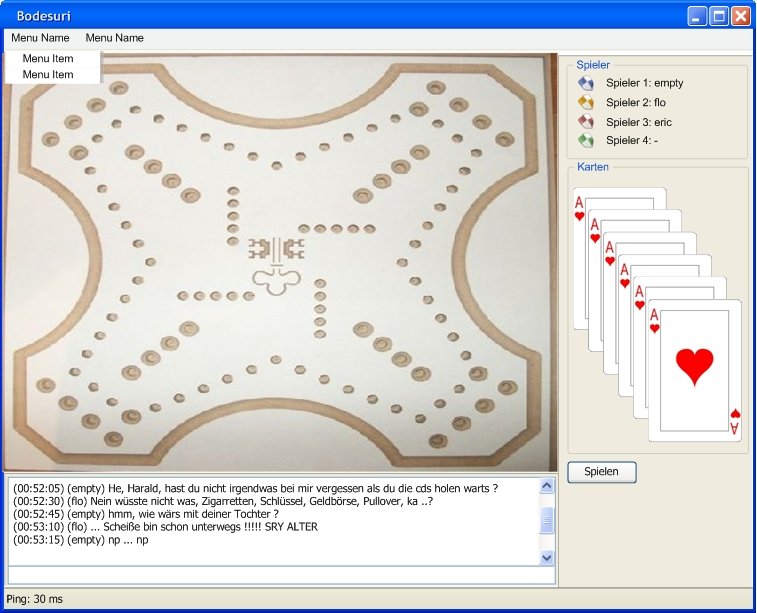
\includegraphics[width=1\textwidth]{Externes_Design.jpg} \caption{Externes Design}\label{fig:Externes_Design.jpg} 
\end{figure}
% subsection externes_design (end)

\subsection{Prozesse \& Threads} % (fold)
\label{sub:prozesse_threads}
Beschrieben, wie diese ablaufen, miteinander funktionieren, Daten austauschen, sich synchronisieren, etc...
% subsection prozesse_threads (end)

% section architektur (end)

\section{Eingeregene Risiken} % (fold)
\label{sec:risiken}

\subsection{RMI} % (fold)
\label{sub:rmi}

Im Verlauf der ersten Tests mit RMI stellte sich schnell heraus, dass RMI weit mehr kann als für das Projekt Notwenig wäre und es dem Projekt somit unnötig Komplexität hinzufügt. Andererseits stellt RMI  einige Anforderungen an die Client/Server Struktur die sich nur schwer mit den Projektanforderungen decken lassen. So kann RMI nur erschwert hinter Firewalls betrieben werden und eine Kommunikation über ein durch NAT\footnote{Network Adress Translation. Firewall-Feature welches Netzbereiche auf andere Netzbereiche zu mappen. Wird häufig verwendet um private Adressbereiche im Internet hinter einer einzelnen Adresse verstecken zu lasssen.} verstecktes Netzwerk ist gar nicht erst möglich. Da die Internet-Zugangslösungen in den meisten Haushalten auf Firewalls und NAT basieren könnte das Spiel von einem grösseren Teil der potentiellen Kundschaft gar nicht gespielt werden.

Wir entschieden uns, auf Grund dieser Probleme, auf eine eigene Lösung umzusteigen welche auf den Java Klassen Socket und Input/OutputObjectStream basidert. Insgesamt gingen etwa 10 Stunden Arbeit für diese Umstellung verloren.

% subsection rmi (end)

\subsection{Java 2D} % (fold)
\label{sub:java_2d}

% subsection java_2d (end)

% section risiken (end)

\end{document}
